\documentclass[11pt]{article}

\usepackage{mathtools}
\usepackage{float}
\usepackage{amssymb}
\usepackage{amsmath}
\usepackage{amsthm}
\usepackage{hyperref}
\usepackage{microtype}
\usepackage{graphicx}
\usepackage{blkarray}
\usepackage{pgfplots}
\pgfplotsset{compat=1.15}
\usepackage{mathrsfs}
\usetikzlibrary{arrows}
\graphicspath{ {./img/} }

\setlength{\parindent}{0cm}
\let\emptyset\varnothing

\title{\textbf{CSCI/MATH 2113 Discrete Structures} \\ Chapter 11 An Introduction to Graph Theory}
\author{Alyssa Motas}

\begin{document}

    \maketitle

    \pagebreak

    \tableofcontents

    \pagebreak

    \section{11.1 Definitions and Examples}

    Let $V$ be a finite nonempty set, and let \(E \subseteq V \times V\). The pair \((V,E)\) is then called a \emph{directed graph} or \emph{digraph}, where $V$ is the set of vertices, or nodes, and $E$ is its set of (directed) edges or arcs. We write \(G = (V,E)\) to denote such a graph.

    \vspace{1em}

    When there is no concern about the direction of any edge, we still write \(G = (V,E)\). But now $E$ is a set of unordered pairs of elements taken from $V$ (cardinality \(\leq 2\)), and $G$ is called an \emph{undirected} graph.

    \vspace{1em}

    Whether \(G = (V,E)\) is directed or undirected, we often call $V$ the vertex set of $G$ and $E$ the edge set of $G$.

    \vspace{1em}

    If \((a,b)\) is an edge in a directed graph, then $a$ and $b$ are the \emph{source} and \emph{target} of the edge. We also say if \(\{a,b\}\) or \((a,b)\), then $a$ and $b$ are \emph{adjacent} and that \(\{a,b\}\) (or \((a,b)\)) is incident to $a$ and $b$. 

    \vspace{1em}

    A loop-free graph is a graph in which no vertex is adjacent to itself.

    \subsection{$x-y$ walk}

    Let \(x,y\) be (not necessarily distinct) vertices in an undirected graph \(G = (V,E)\). An \(x-y\) \emph{walk} in $G$ is a (loop-free) finite alternating sequence \[x = x_0, e_1, x_1, e_2, x_2, e_3, \dots, e_{n-1}, x_{n-1}, e_n, x_n = y\] of vertices and edges from $G$, starting at vertex $x$ and ending at vertex $y$ and involving the $n$ edges \(e_i = \{x_{i-1}, x_i\}\), where \(1 \leq i \leq n\). 

    \vspace{1em}

    The \emph{length} of this walk si $n$, the number of edges in the walk. (When \(n=0\), there are no edges; \(x =y\), and the walk is called \emph{trivial}).

    \vspace{1em}

    Any \(x-y\) walk where \(x=y\) (and \(n>1\)) is called a \emph{closed walk}. Otherwise, the walk is called \emph{open}.

    \subsection{Example of a walk}

    \begin{figure}[H]
        \centering
        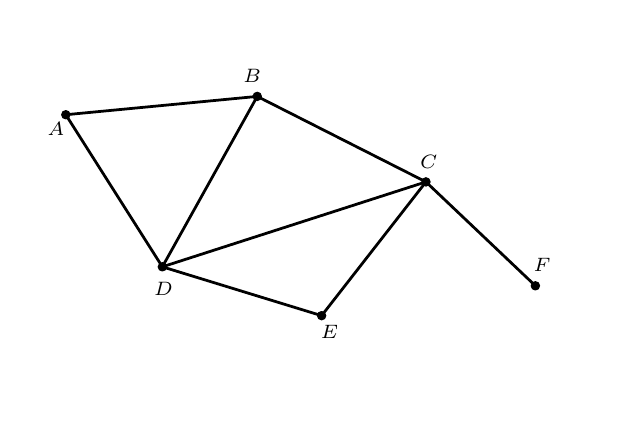
\begin{tikzpicture}[line cap=round,line join=round,>=triangle 45,x=1cm,y=1cm, scale=1.5]
            \clip(-2.1972312014361104,-0.7531236698191296) rectangle (2.5529337524641975,2.3516943247823425);
            \draw [line width=1pt] (-1.8743029335374306,1.6146562438016798)-- (-0.2534974439644721,1.7697441337393276);
            \draw [line width=1pt] (-0.2534974439644721,1.7697441337393276)-- (-1.0568532083615039,0.3269567940163623);
            \draw [line width=1pt] (-1.0568532083615039,0.3269567940163623)-- (-1.8743029335374306,1.6146562438016798);
            \draw [line width=1pt] (-1.0568532083615039,0.3269567940163623)-- (1.1746905816302509,1.046000647363638);
            \draw [line width=1pt] (1.1746905816302509,1.046000647363638)-- (-0.2534974439644721,1.7697441337393276);
            \draw [line width=1pt] (-1.0568532083615039,0.3269567940163623)-- (0.29146903948614583,-0.08661091248403163);
            \draw [line width=1pt] (0.29146903948614583,-0.08661091248403163)-- (1.1746905816302509,1.046000647363638);
            \draw [line width=1pt] (1.1746905816302509,1.046000647363638)-- (2.101387680257573,0.16634266378856072);
            \begin{scriptsize}
            \draw [fill=black] (-1.8743029335374306,1.6146562438016798) circle (1pt);
            \draw[color=black] (-1.958482701794907,1.4964264110106556) node {$A$};
            \draw [fill=black] (-0.2534974439644721,1.7697441337393276) circle (1pt);
            \draw[color=black] (-0.2965450939028932,1.9445637132765076) node {$B$};
            \draw [fill=black] (1.1746905816302509,1.046000647363638) circle (1pt);
            \draw[color=black] (1.197958501253731,1.2125586715922444) node {$C$};
            \draw [fill=black] (-1.0568532083615039,0.3269567940163623) circle (1pt);
            \draw[color=black] (-1.0468975213466756,0.14097639738343962) node {$D$};
            \draw [fill=black] (0.29146903948614583,-0.08661091248403163) circle (1pt);
            \draw[color=black] (0.3576878077113137,-0.2219244071803688) node {$E$};
            \draw [fill=black] (2.101387680257573,0.16634266378856072) circle (1pt);
            \draw[color=black] (2.1591537595494854,0.34097639738343962) node {$F$};
            \end{scriptsize}
            \end{tikzpicture}
    \end{figure}
    \(\{a,b\},\{b,d\}, \{d,c\}, \{c,e\}, \{e,d\}, \{d,b\}\) is an \(a-b\) walk. This walk has length 6.

    \subsection{Trail, circuit, path, and cycles}
 
    An \(x-y\) walk is a \emph{trail} if no edge is repeated. A closed trail is a \emph{circuit}. A \emph{path} is a trail in which no vertex occurs more than once. A closed path is a \emph{cycle}. (=trail where the only repeated vertices are the first and last one). 

    \vspace{1em}

    \emph{Theorem:} Let \(G = (V,E)\) be an undirected graph. Let \(a,b \in V\) with \(a \neq b\). If there is a trail between $a$ and $b$ then there is a path between $a$ and $b$.

    \begin{proof}
        Suppose there is a trail from $a$ to $b$. Take one of smallest length.
        \begin{itemize}
            \item If the trail is a path, we are done.
            \item If not, then it is of the form \[\{a,x_1\}, \{x_1, x_2\}, \dots,  \{x_{k-1}, x_k\}, \{x_{k+1}, x_{k+2}\}, \dots, \{x_{m-1}, x_m\}, \{x_m, x_{m+1}\}, \dots, \{x_m, b\}\] where \(x_k = x_m\). But then \[\{a_, x_1\}, \{x_1, x_2, \dots, \{x_{k-1}\}, x_k\}, \{x_m, x_{m+1}\}, \dots, \{x_n,b\}\] is a shorter trail from $a$ to $b$ which is a contradiction.
        \end{itemize}
    \end{proof}

    \begin{center}
        \begin{tabular}{| c | c | c | c | c |} \hline
            Repeated Vertex & Repeated & & & \\ 
            (Vertices) & Edge(s) & Open & Closed & Name \\ \hline
            Yes & Yes & Yes & & Walk (open) \\
            Yes & Yes & & Yes & Walk (closed) \\
            Yes & No & Yes & & Trail \\
            Yes & No & & Yes & Circuit \\
            No & No & Yes & & Path \\
            No & No & & Yes & Cycle \\ \hline
        \end{tabular}
    \end{center}

    \subsection{Connect and disconnect}

    A graph $G$ is \emph{connected} if there is a path between any two distinct vertices of $G$. A graph that is not connected is \emph{disconnected}. 

    \vspace{1em}

    For any graph \(G = (V,E)\), the number of (connected) components of $G$ is denoted by \(\kappa (G)\). 

    \subsection{Multigraph}

    Let $V$ be a set (non-empty). Then \((V,E)\) is a \emph{multigraph} if there are \(a,b \in V\) such that $E$ contains more than one edge between $a$ and $b$. (Strictly speaking, $E$ is a multiset (set with repetition)). 

    \begin{figure}[H]
        \centering
        \includegraphics[scale=0.2]{multigraph.png}
    \end{figure}
    Here, the edge \((a,c)\) has \emph{multiplicity} 2.

    \section{Subgraphs, Complements and Graph Isomorphism}

    \subsection{Subgraph}

    If \(G = (V,E)\) is a graph (directed or undirected), then \(G_1 = (V_1, E_1)\) is called a \emph{subgraph} of $G$ if \(\emptyset \neq V_1 \subseteq V\) and \(E_1 \subseteq E\), where each edge in \(E_1\) is incident with vertices in \(V_1\).

    \begin{figure}[H]
        \centering
        \includegraphics[scale=0.2]{subgraph.png}
    \end{figure}

    Note that $G_1$ is a subgraph of $G_2$.

    \subsection{Spanning subgraph}

    If \(G = (V,E)\) and \(G_1 = (V_1, E_1)\) and \(G_1\) is a subgraph of $G$, then \(G_1\) is a \emph{spanning} subgraph if \(V_1 = V\).

    \begin{figure}[H]
        \centering
        \includegraphics[scale=0.2]{spanning.png}
    \end{figure}
    \(G_1, G_2\) are subgraphs of $G$ and \(G_2\) is a spanning subgraph of $G$.

    \subsection{Induced subgraph}

    Let \(G = (V,E)\) and \(V' \subseteq V\) with \(V' \neq \emptyset\). The subgraph \emph{induced} by \(V'\) is the subgraph whose vertex set is \(V'\) and whose edge set contains all of the edges of $E$ between elements of \(V'\). We denote this subgraph by \(\langle v' \rangle\).

    \subsubsection{Example}

    \begin{figure}[H]
        \centering
        \includegraphics[scale=0.2]{induced.png}
    \end{figure}

    \subsection{Deleted vertex or edge}

    Let \(G = (V,E)\) be a graph and let \(w \in V\). Then \[G - w = (V', E')\] where \[V' = V \setminus \{w\}\] and $E'$ contains all the edges in $E$ except those incident to $w$.

    \subsection{Complete graph}

    Let $V$ be a set of \(n \geq 1\) vertices. The \emph{complete graph} on $n$ vertices is denoted \(K_n\) and has $V$ as vertices and all edges \(\{a,b\}\) for \(a,b \in V\).

    \subsection{Complement}

    Let $G$ be a graph with \(G = (V,E)\). The \emph{complement} of $G$, written \(\overline{G}\), has the same vertices as $G$ but all of the edges not in $G$.

    \subsection{Comparing graphs}

    \begin{figure}[H]
        \centering
        \includegraphics[scale=0.2]{triangle1.png}
    \end{figure}

    are two ways of representing the same graph (different embeddings in the plane). However

    \begin{figure}[H]
        \centering
        \includegraphics[scale=0.2]{triangle2.png}
    \end{figure}

    is a different graph. But they are \emph{isomorphic}.

    \subsection{Homomorphism and isomorphism}

    Let \(G_1 = (V_1, E_1)\) and \(G_2 = (V_2, E_2)\) be two graphs. A function \[f:V_1 \rightarrow V_2\] which satisfies: \[\text{$a$ and $b$ adjacent in $G_1$ implies $f(a)$ and $f(b)$ adjacent in $G_2$}\] is called a graph \emph{homomorphism}. If $f$ is also a bijection, then $f$ is a graph \emph{isomorphism}. When there is an isomorphism between \(G_1\) and \(G_2\), we say that \(G_1\) and \(G_2\) are \emph{isomorphic}.

    \subsubsection{Examples of isomorphism}

    \begin{figure}[H]
        \centering
        \includegraphics[scale=0.2]{iso1.png}
    \end{figure}

    are isomorphic since \(a \rightarrow w, b \rightarrow x, c \rightarrow y, d \rightarrow z\) is an isomorphism. Here, any bijection \(\{a,b,c,d\} \rightarrow \{w,x,y,z\}\) would do.

    \begin{figure}[H]
        \centering
        \includegraphics[scale=0.2]{iso2.png}
    \end{figure}

    are isomorphic since \(m \rightarrow s, q \rightarrow t, n \rightarrow r, p \rightarrow u\) is an isomorphism.

    An example of a graph homomorphism that is not an isomorphism:
    \begin{figure}[H]
        \centering
        \includegraphics[scale=0.2]{homo1.png}
    \end{figure}

    The function \(a \rightarrow k, b \rightarrow l, c \rightarrow i, d \rightarrow j\) is such an example.

    \vspace{1em}

    Are the graphs below isomorphic?

    \begin{figure}[H]
        \centering
        \includegraphics[scale=0.2]{iso3.png}
    \end{figure}

    Yes, for example: \(a \rightarrow q, c \rightarrow u, e \rightarrow r, g \rightarrow x, i \rightarrow z, b \rightarrow v, f \rightarrow w, u \rightarrow t, j \rightarrow s\).

    \pagebreak

    What about these graphs?
    \begin{figure}[H]
        \centering
        \includegraphics[scale=0.2]{iso4.png}
    \end{figure}

    Nope. In the left graph, $a$ and $d$ are adjacent to 2 vertices and all other vertices are adjacent to 4 vertices. This is not the case in the right graph.

    \vspace{1em}

    \emph{Remark:} There currently is no method to decide efficiently if two graphs are isomorphic.

    \section{11.3 Vertex Degree: Euler Trails and Circuits}

    \subsection{Degree}

    In an undirected graph (multigraph), the \emph{degree} of a vertex $v$, written deg($v$), is the number of edges incident to $v$. (A loop is considered as 2 edges incident to $v$).

    \vspace{1em}

    \emph{Example:}
    \begin{figure}[H]
        \centering
        \includegraphics[scale=0.1]{deg.png}
    \end{figure}
    We have \(\deg(a) = \deg(b) = \deg(d) = 3, \deg(c)=2, \deg(e)=1, \deg(f) = 0\). Since $e$ has degree 1, it is called a \emph{pendant} vertex.

    \subsection{Sum of degrees}

    If \(G = (V,E)\) is an undirected graph (or multigraph), then \[\sum_{v \in V} \deg(v) = 2 \cdot |E|.\]

    \begin{proof}
        By induction.
        \begin{itemize}
            \item \(|E| = 0\) then the equality holds.
            \item \(|E| = 1\) then we have \[* \dots * (\deg 0) * - * (\deg 1)\] so \(\sum \deg(v) = 2 = 2 |E|\) and the equality holds. 
            \item \(|E| = n+1\) then \(E = \{\{a,b\}\} \cup E'\). Consider \(G' = (V,E')\). By the induction hypothesis: \[\sum_{v \in V} \deg(v) \in G' = 2|E'|.\] Then 
            \begin{align*}
                \sum_{v \in V} \deg(v) &= \sum_{v \in V} \deg(v) + 2 \\
                                       &= 2 |E'| + 2\\
                                       &= 2 |E|.
            \end{align*}
        \end{itemize}
    \end{proof}

    \emph{Corollary:} The number of vertices of odd degree is even.
    \begin{proof}
        By considering the equality in the previous theorem modulo 2.
    \end{proof}

    \subsection{$k$-regular}

    A graph is $k$-regular if all of its vertices have degree $k$.
    \begin{figure}[H]
        \centering
        \includegraphics[scale=0.2]{kregular.png}
    \end{figure}

    \emph{Claim:} There is no 4-regular graph with 15 edges. Indeed, if a graph is 4-regular then \[\sum_{v \in V} \deg(v) = 4 |V|\] and if there are 15 edges then \[2|E| = 30\] but \(4|V| = 30\) has no integer solution.

    \vspace{1em}

    \emph{Another example:} 4-regular graph with 10 edges exist:
    \begin{figure}[H]
        \centering
        \includegraphics[scale=0.1]{4reg.png}
    \end{figure}

    \subsection{The seven bridges of Konigsberg}

    A map of Konigsberg:
    \begin{figure}[H]
        \centering
        \includegraphics[scale=0.2]{konigsberg.png}
    \end{figure}

    Can you walk along all the bridges, using each bridge only once?

    \subsection{Euler circuit and trail}

    Let \(G = (V,E)\) be an undirected graph or multigraph with no isolated vertices. Then $G$ has an \emph{Euler circuit} if there is a circuit in $G$ that traverses every edge. An \emph{Euler trail} is an open trail that traverses every edge. 

    \subsection{Euler circuit and trail condition}

    Let $G$ be an undirected graph or multigraph with no isolated vertices. Then $G$ has an Euler circuit if and only if $G$ is connected and every vertex in $G$ has even degree.

    \begin{proof}
        \(\Rightarrow\) If $G$ has an Euler circuit then it is connected. Moreover, every time the circuit reaches a node it must leave that node along another edge. Hence, the degree is even.
    \end{proof}

    \emph{Corollary:} If $G$ is an undirected graph or multigraph, then $G$ has an Euler trail if and only if $G$ is connected and exactly two vertices have odd degree.

    \emph{Remark:} The Konigsberg graph has 4 nodes of odd degree.

    \pagebreak

    \section{11.4 Planar Graphs}

    \subsection{Definition of planar}

    A graph $G$ is \emph{planar} if $G$ can be drawn in the plane with its edges intersecting only at vertices.

    (Recall: a drawing of $G$ in the plane is an embedding.) A graph is planar if it has a planar embedding.
    \begin{figure}[H]
        \centering
        \includegraphics[scale=0.3]{planar.png}
    \end{figure}

    \subsection{Bipartite}

    A graph \(G = (V,E)\) is \emph{bipartite} if \(V = V_1 \cup V_2\) with \(V_1 \cap V_2 = \emptyset\) and every edge in $G$ is of the form \(\{a,b\}\) where \(a \in V_1\) and \(b \in V_2\). If every vertex in \(V_1\) is adjacent to every vertex in \(V_2\) then the graph is a \emph{complete bipartite} graph (denoted \(K_{|V_1|,|V_2|}\)).

    \subsubsection{Examples}

    \begin{figure}[H]
        \centering
        \includegraphics[scale=0.2]{bipartite.png}
    \end{figure}

    We know that \(K_5\) and \(K_{3,3}\) are not planar. As a result, if a graph $G$ has \(K_5\) or \(K_{3,3}\) as a subgraph, then $G$ is not planar.

    \subsection{Elementary subdivision}

    Let \(G = (V,E)\) be loop-free and undirected with \(E \neq \emptyset\). An \emph{elementary subdivision} of $G$ is obtained by removing an edge \(\{a,b\}\) from $E$ and adding the edges \(\{a,c\}\) and \(\{c,b\}\) to $E$ and adding $c$ in $V$ (where \(c \notin V\)). 

    \subsubsection{Example}

    \begin{figure}[H]
        \centering
        \includegraphics[scale=0.2]{elemsub.png}
    \end{figure}

    Here, $G_1$ is obtained through an elementary subdivision of $G$. Similarly, $G_2$ is obtained from $G_1$ (and from $G$ as well). 

    \vspace{1em}

    \emph{Remark:} If \(G'\) is obtained from $G$ by a single elementary subdivision then \[|V'| = |V| + 1 \quad \text{and} \quad |E'| = |E| + 1.\]

    \emph{Definition:} If $G$ and $G'$ are two graphs such that $G$ and $G'$ can be obtained from the same graph through a sequence of elementary subdivisions.

    \subsection{Nonplanar homeomorphic property}

    A graph is nonplanar if and only if it contains a subgraph that is homeomorphic to \(K_5\) or \(K_{3,3}\).

    \begin{figure}[H]
        \centering
        \includegraphics[scale=0.2]{homo2.png}
    \end{figure}
    Hence, the graph above is not planar.

    \subsection{Regions}

    We can count the number of regions in the plane determined by a (planar embedding) of a planar graph.

    \begin{figure}[H]
        \centering
        \includegraphics[scale=0.2]{region.png}
    \end{figure}

    \emph{Theorem:} Let \(G = (V,E)\) be a planar graph. Let $r$ be the number of regions in the plane determined by $G$. Then \[|V| - |E| + r = 2.\]

    \emph{Corollary:} For a connected loop-free planar graph with more than 2 edges, we have \[3r \leq 2e \quad \text{and} \quad e \leq 3v - 6.\]

    \emph{Example:} \(K_5\) has 10 edges and 5 vertices, so \[3|V| - 6 = 15 - 6 = 9 \leq 10 = e.\] Hence, \(K_5\) is not planar.

    \section{11.6 Graph Coloring and Chromatic Polynomials}

    \subsection{Proper colouring}

    If \(G = (V,E)\) is an undirected graph, a \emph{proper colouring} of $G$ occurs when we color the vertices of $G$ so that if \(\{a,b\}\) is an edge in $G$, then $a$ and $b$ are coloured with different colors. (Hence adjacent vertices have different colors.)

    \subsubsection{Example:}
    \begin{figure}[H]
        \centering
        \includegraphics[scale=0.2]{proper.png}
    \end{figure}

    \emph{Remark:} We can think of a colouring as a function \[c:V \rightarrow \text{Colours}\] where Colours is a set of colours. 

    \subsection{Chromatic Number}

    The minimum number of colors needed to properly colour $G$ is called the \emph{chromatic number} of $G$ and is written \(\chi(G)\).

    \subsubsection{Example}

    \begin{figure}[H]
        \centering
        \includegraphics[scale=0.2]{chromno.png}
    \end{figure}
    We have \(\chi (G) = 3\). 

    \vspace{1em}

    Another example is: \(\chi (K_n) = n\).

    \subsection{Chromatic Polynomial}

    Let $G$ be a graph and let $\lambda$ be the number of available colours. We write \[P(G, \lambda)\] for the number of ways that we could properly colour $G$ using \(\lambda\) colours. 

    \emph{Note:} \[\color{green}{a} \color{black} \rightarrow \color{red} b \qquad \color{red} a \color{black} \rightarrow \color{green} b\] are different colourings.

    \subsection{Examples}

    \begin{itemize}
        \item Let \(G = (\{a_1, \dots, a_n\}, \emptyset)\). So, we have for $G$: \[a_1 \quad a_2 \quad \dots \quad a_n\] What is \(P(G, \lambda)\)? We have \(\lambda\) options for \(a_1\), \(\lambda\) options for \(a_2\), \dots Hence, \(P(G,\lambda) = \lambda^{n}\).
        \item What is \(P(K_n, \lambda)\)? For the 1st vertex: \(\lambda\) and for the 2nd: \(\lambda - 1\). So, \[P(K_n,\lambda) = \lambda \cdot (\lambda - 1)(\lambda -2) \dots (\lambda - n + 1) = \lambda^{(n)}.\] Note that if \(\lambda < n\) then \[P(G,\lambda) = 0.\] Note also that \(\lambda=n\) is the smallest integer for which \[P(G,\lambda) > 0\] which is \(\chi (G)\). 
        \item For a graph $G$, we have 
        \begin{figure}[H]
            \centering
            \includegraphics[scale=0.1]{poly1.png}
        \end{figure}
        which is \(P(G,\lambda) = \lambda(\lambda - 1)^3.\) More generally, for a path $G$ on $n$ vertices, we have \[P(G,\lambda) = \lambda (\lambda - 1)^{n-1}.\]
    \end{itemize}

    \pagebreak

    \emph{Remark:}
    \begin{figure}[H]
        \centering
        \includegraphics[scale=0.2]{poly2.png}
    \end{figure}
    We have \(P(G,\lambda) = P(G_1, \lambda) \cdot P(G_2, \lambda)\). 
    
    \subsection{Coalescing vertices}
    
    Let \(G=(V,E)\) be an undirected graph. For \(e = \{a,b\} \in  E\), let $G_e$ denote the subgraph of $G$ obtained by deleting $e$ from $G$, without removing vertices $a$ and $b$; that is, \[G_e = G - e.\] From $G_e$, a second subgraph of $G$ is obtained by coalescing (or, identifying) the vertices $a$ and $b$. This second subgraph is denoted by \(G'e\).
    
    \subsubsection{Example}

    \begin{figure}[H]
        \centering
        \includegraphics[scale=0.2]{ge.png}
    \end{figure}

    \subsection{Decomposition Theorem for Chromatic Polynomials}

    If \(G = (V,E)\) is a connected graph and \(e \in E\), then \[P(G_e, \lambda) = P(G, \lambda) + P(G'_e, \lambda).\]

    \begin{proof}
        Let \(e = \{a,b\}\). Consider a proper colouring of \(G_e\). Either $a$ and $b$ have the same colour or not. In the first case we have a colouring of \(G'_e\) and in the second case a colouring of $G$. hence, a colouring of \(G_e\) is either a colouring of $G$ or a colouring of \(G'_e\). 
    \end{proof}

    \subsubsection{Examples}

    Write \([G]\) for the chromatic polynomial fo $G$. 
    \begin{figure}[H]
        \centering
        \includegraphics[scale=0.2]{decom1.png}
    \end{figure}
    We have
    \begin{align*}
        G &= G_e - G'_e \\
          &= P(G_e, \lambda) - P(G'_e,\lambda) \\
          &= \lambda (\lambda - 1)^3 - \lambda^{(3)} \\
          &= \lambda^4 - 4\lambda^3 + 6 \lambda^2 - 3\lambda.
    \end{align*}
    Then, we have \(P(G,\lambda) > 0\) if and only if \(\lambda \geq 2\) so \(\chi (G) = 2\). 
    
    \pagebreak

    Another example:
    \begin{figure}[H]
        \centering
        \includegraphics[scale=0.2]{decom2.png}
    \end{figure}
    Then we have \[= \lambda (\lambda^{(4)}) - 2(\lambda^{(4)}) = \lambda(\lambda - 1)(\lambda - 2)^2 (\lambda - 3)\]

    \subsection{Constant term}

    For every graph $G$, the constant term of \(P(G, \lambda)\) is 0.
    \begin{proof}
        Evaluating \(P(G,\lambda)\) at 0 gives the constant term of the polynomial. But there is no way to show a graph with 0 colours, so this term must be 0.
    \end{proof}

    \subsection{Sum of the coefficients}

    If \(G = (V,E)\) and \(|E| > 0\) then the sum of the coefficients in \(P(G,\lambda)\) is 0.

    \begin{proof}
        Evaluating \(P(G, \lambda)\) at 1 yields the sum of the coefficients. But $G$ has at least one edge so 2 or more colours are needed to colour $G$. Hence, \(P(G,\lambda)\) must be 0 when evaluated at 1.
    \end{proof}

    \subsection{Addition of an edge}

    Let \(G = (V,E)\) with \(a,b \in V\) and \(\{a,b\} \notin E\). Adding the edge \(\{a,b\}\) gives \(G_e^+\) and identifying $a$ and $b$ in $G$ gives \(G_e^{++}\). Then \[P(G,\lambda) = P(G_e^+,\lambda) + P(G_e^{++},\lambda). \]

    \subsection{Union and intersection}

    Let \(G_1 = (V_1, E_1)\) and \(G_2 = (V_2, E_2)\) be two graphs. Then
    \begin{itemize}
        \item the \emph{union} of \(G_1\) and \(G_2\) is the graph \(G_1 \cup G_2 = (V,E)\) where \(V = V_1 \cup V_2\), \(E = E_1 \cup E_2\).
        \item (when \(V_1 \cap V_2 \neq \emptyset\)) the \emph{intersection} of \(V_1\) and \(V_2\) is the graph \(G_1 \cap G_2 = (V,E)\) where \(V = V_1 \cap V_2\), \(E = E_1 \cap E_2\).
    \end{itemize}

    \subsection{Ways to properly color \(K_n\)}

    Let $G$ be an undirected graph with subgroups \(G_1, G_2\). If \(G = G_1 \cup G_2\) and \(G_1 \cap G_2 = K_n\) for some $n$ then \[P(G,\lambda) = \frac{P(G_1, \lambda) \cdot P(G_2, \lambda)}{\lambda^{(n)}}\]
\end{document}